
\chapter{New use cases}
\label{ch:newCases}


%%%%%%%%%%%%%%%%%%%%%%%%%%%%%%%%%%%%%%%%%%%%%%%%%%%%%%%%
\section{Handling IOV in optimal design models}
\label{sec:IOVinODE}
New challenges occurred when we started to encode the optimal design 
test cases with inter-occasion (aka between-occasion) variability. It turns out
there are several ways to encode it, depending on what type of mapping is 
used and where it is implemented. For this discussion we consider a standard
setup illustrated in Figure \ref{fig:IOVdesign} with two arms, two occasions and design 
related covariates: treatments and sequence of treatments.

\begin{figure}[htb]
\centering
  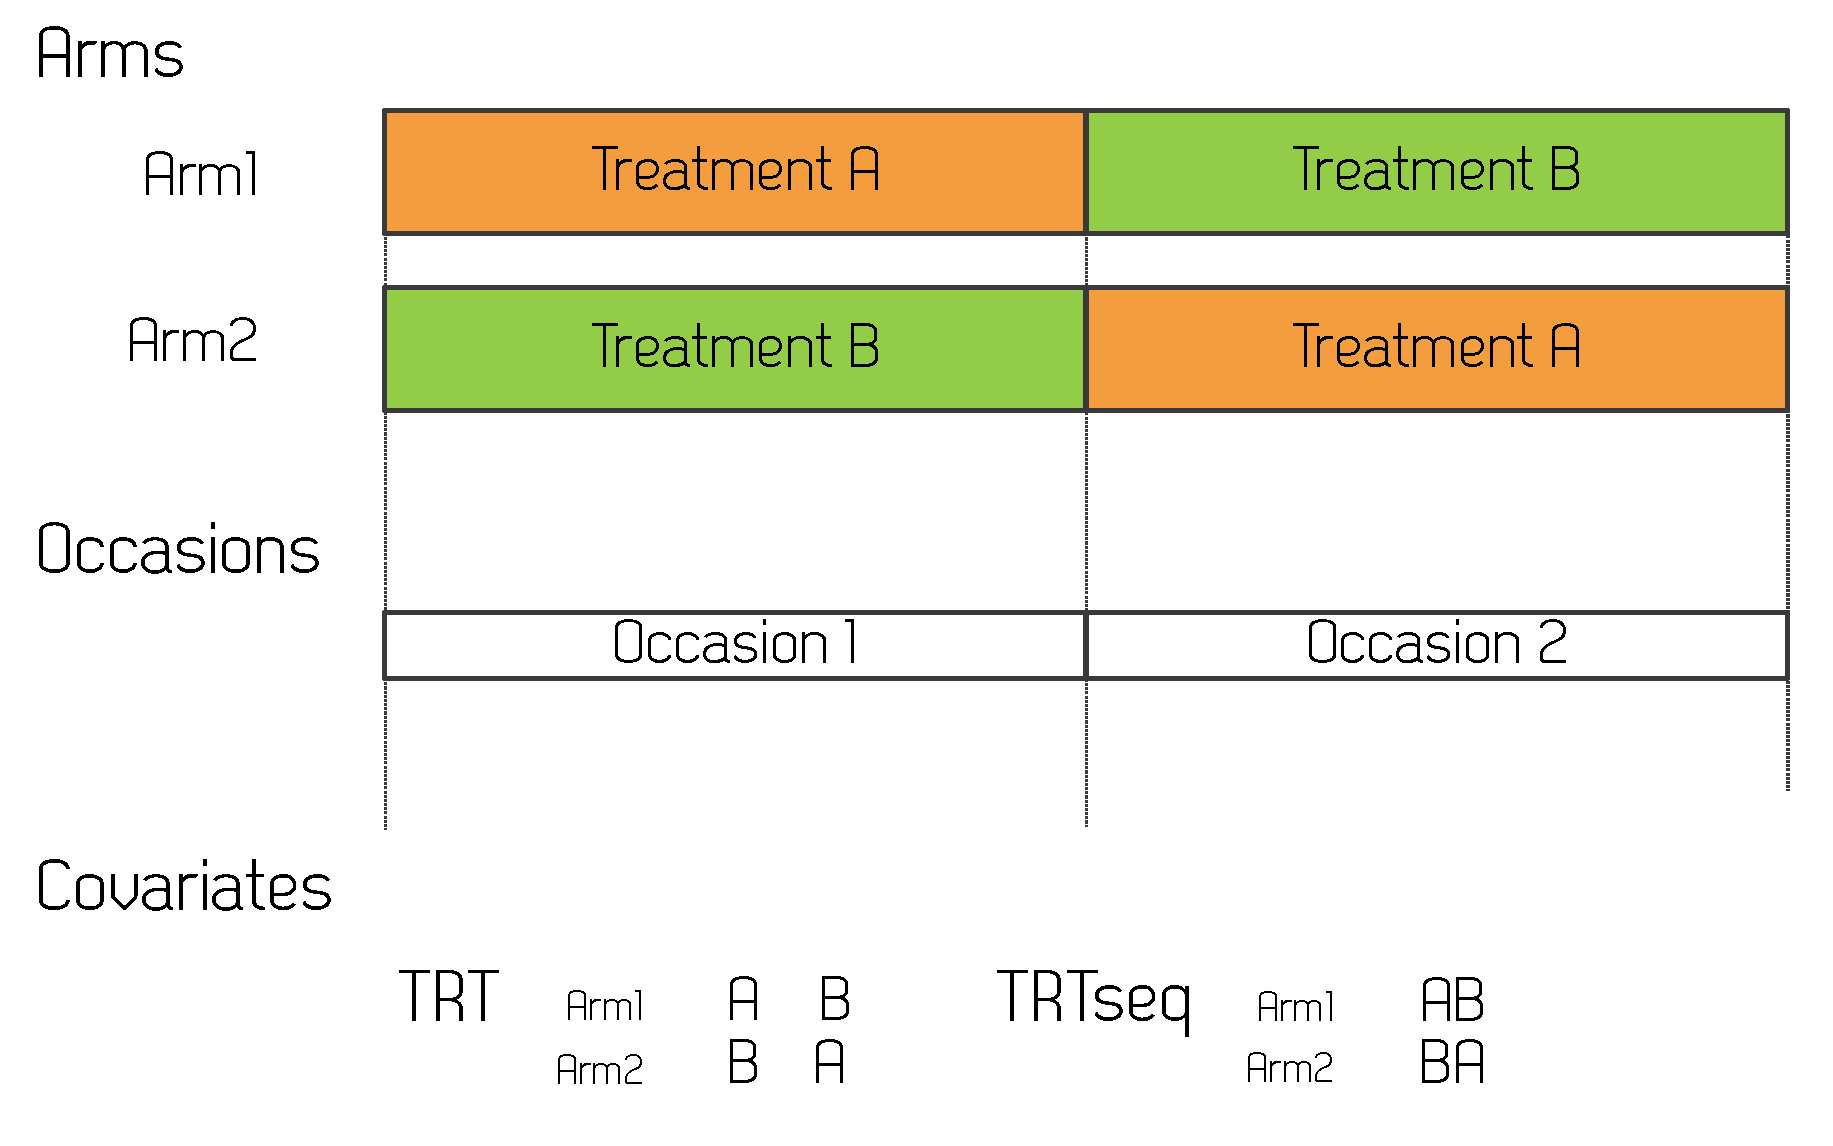
\includegraphics[width=140mm]{pics/IOVexample}
  \caption{IOV with design related covariates.}
  \label{fig:IOVdesign}
\end{figure}


%%%%%%%%%%%%%%%%%%%%
\subsection{Implementation options}
\begin{description}
\item[Option 1] Association of covariates-occasions within arms
\item[Option 2] Arm-specific occasions declaration and association with covariates
\item[Option 3] Covariates and occasions declared in the top level
\item[Option 4] Covariates and occasions declared in \xelem{IndividualCovariates}
\end{description}



%%%%%%%%%%%%%%%%%%%%
\subsection{Option 1}
Define 
\begin{itemize}
\item 
occasions for all arms in the top level of \xelem{TrialDesign} with IOV reference
\lstset{language=XML}
\begin{lstlisting}
    <Occasions>
        <OccasionList oid="ol1">
            <ct:VariabilityReference>
                <ct:SymbRef blkIdRef="vm_mdl" symbIdRef="OCC"/>
            </ct:VariabilityReference>
            <Occasion oid="OCC_1">
                <Start>
                    <ct:Assign>
                        <ct:Int>0</ct:Int>
                    </ct:Assign>
                </Start>
            </Occasion>
            <Occasion oid="OCC_2">
                <Start>
                    <ct:Assign>
                        <ct:Int>120</ct:Int>
                    </ct:Assign>
                </Start>
            </Occasion>
        </OccasionList>
    </Occasions>
\end{lstlisting}
\item
the occasion sequence is then referenced from each arm
\lstset{language=XML}
\begin{lstlisting}
            <Arm oid="arm1">
	        <CovariateModel>
                    <!-- omitted details -->
	        </CovariateModel>
                <InterventionSequence>
                    <!-- omitted details -->
                </InterventionSequence>
                <ObservationSequence>
                    <!-- omitted details -->
                </ObservationSequence>
                
                <OccasionSequence>
                    <OccasionListRef oidRef="ol1"/>
                </OccasionSequence> 
            </Arm>
\end{lstlisting}
\item
declare also the \xatt{TRT} covariate in each arm and associate its categories with occasions
\lstset{language=XML}
\begin{lstlisting}
	<Arms>
	    <Arm oid="arm1">
	        <CovariateModel oid="arm1_td_cm">
		    <CovariateModelRef oidRef="cm"/>
		    <Covariate symbId="TRT">
		        <mdef:Categorical>
			    <mdef:Category catId="A">
			        <mdef:OccasionRef oidRef="OCC_1"/>
			    </mdef:Category>
			    <mdef:Category catId="B">
				<mdef:OccasionRef oidRef="OCC_2"/>
			    </mdef:Category>
		        </mdef:Categorical>
	             </Covariate>
		     <Covariate symbId="TRTseq">
		         <mdef:Categorical>
		             <mdef:Category catId="AB"/>
		         </mdef:Categorical>
		     </Covariate>
		</CovariateModel>
\end{lstlisting}
\end{itemize}


%%%%%%%%%%%%%%%%%%%%
\subsection{Option 2} 

\begin{itemize}
\item 
Declare arm-specific occasions (even though they are defined on the 
same time intervals) with different object identifiers, \xatt{oid}, 
e.g. \textit{arm1\_OCC\_1} and \textit{arm1\_OCC\_2} for arm 1 
\lstset{language=XML}
\begin{lstlisting}
<Arms>
    <Arm oid="arm1">
	<OccasionSequence>
	    <OccasionList oid="arm1_OCC">
	        <ct:VariabilityReference>
	            <ct:SymbRef blkIdRef="vm_mdl" symbIdRef="OCC"/>
	        </ct:VariabilityReference>
	        <Occasion oid="arm1_OCC_1">
	            <Start>
	                <ct:Assign>
	                    <ct:Int>0</ct:Int>
	                </ct:Assign>
	            </Start>
	        </Occasion>
	        <Occasion oid="arm1_OCC_2">
	            <Start>
	                <ct:Assign>
	                    <ct:Int>120</ct:Int>
	                </ct:Assign>
	            </Start>
	        </Occasion>
            </OccasionList>
	</OccasionSequence>
    </Arm>
\end{lstlisting}
\item
associate these occasions to categories as well in each arm
\lstset{language=XML}
\begin{lstlisting}
	<CovariateModel oid="arm2_td_cm">
	    <CovariateModelRef oidRef="cm"/>
	    <Covariate symbId="TRT">
	        <mdef:Categorical>
		    <mdef:Category catId="B">
		        <mdef:OccasionRef oidRef="arm2_OCC_1"/>
		    </mdef:Category>
		    <mdef:Category catId="A">
			<mdef:OccasionRef oidRef="arm2_OCC_2"/>
		    </mdef:Category>
		</mdef:Categorical>
	    </Covariate>
	    <Covariate symbId="TRTseq">
		<mdef:Categorical>
		    <mdef:Category catId="BA"/>
		</mdef:Categorical>
	    </Covariate>
	</CovariateModel>
\end{lstlisting}
\end{itemize}


%%%%%%%%%%%%%%%%%%%%
\subsection{Option 3}

In this case occasions are defined in the top trial design level and
their sequences referenced in each arm. Also the covariate model 
is located in the top level with
\begin{itemize}
\item 
the TRT covariate is associated with administrations, here \xatt{admin1}
and \xatt{admin2}
\lstset{language=XML}
\begin{lstlisting}
		<Covariates>
		    <CovariateModel oid="td_cm">
		        <CovariateModelRef oidRef="cm"/>
		        <Covariate symbId="TRT">
	                    <mdef:Categorical>
			        <mdef:Category catId="B">
		                    <mdef:InterventionRef oidRef="admin1"/>
			        </mdef:Category>
			        <mdef:Category catId="A">
			            <mdef:InterventionRef oidRef="admin2"/>
			        </mdef:Category>
			    </mdef:Categorical>
		        </Covariate>
\end{lstlisting}
\item
while the \xatt{TRTseq} covariate declared conditional on arms
\lstset{language=XML}
\begin{lstlisting}
			<Covariate symbId="TRTseq">
			    <mdef:Categorical>
			        <ct:Assign>
				    <math:Piecewise>
				        <math:Piece>
					    <ct:CatRef catIdRef="AB"/>
					    <math:Condition>
					        <math:LogicBinop op="eq">
						    <StudyArm/>
						    <ct:OidRef oidRef="arm1"/>
						</math:LogicBinop>
					    </math:Condition>
					</math:Piece>
					<math:Piece>
					    <ct:CatRef catIdRef="BA"/>
					    <math:Condition>
					        <math:LogicBinop op="eq">
						    <StudyArm/>
						    <ct:OidRef oidRef="arm2"/>
						</math:LogicBinop>
					</math:Condition>
				    </math:Piece>
				</math:Piecewise>
			    </ct:Assign>
			</mdef:Categorical>
		    </Covariate>
	        </CovariateModel>
	    </Covariates>
\end{lstlisting}
\end{itemize}

%%%%%%%%%%%%%%%%%%%%
\subsection{Option 4}

This case  is different from the previous ones in that the \xelem{IndividualCovariates}
is used and the relevant design characteristic are stored within inline 
dataset. The following code snippet shows the columns definition and complete 
data record

\lstset{language=XML}
\begin{lstlisting}
<Covariates>
    <IndividualCovariates oid="ic1">
        <ds:DataSet>
            <ColumnMapping>
            <!-- see below -->
            </ColumnMapping>
            <ds:Definition>
                <ds:Column columnId="ARM" columnType="arm" valueType="id" columnNum="1"/>
                <ds:Column columnId="TIME" columnType="time" valueType="real" columnNum="2"/>
                <ds:Column columnId="OCC" columnType="varLevel" valueType="string" columnNum="3"/>
                <ds:Column columnId="TRT" columnType="covariate" valueType="string" columnNum="4"/>
                <ds:Column columnId="TRTseq" columnType="covariate" valueType="string" columnNum="5"/>
            </ds:Definition>
            <ds:Table>
                <ds:Row>
	            <ct:Id>arm1</ct:Id><ct:Real>0</ct:Real><ct:String>occ1</ct:String><ct:String>A</ct:String><ct:String>AB</ct:String>
	            <ct:Id>arm1</ct:Id><ct:Real>119</ct:Real><ct:String>occ1</ct:String><ct:String>A</ct:String><ct:String>AB</ct:String>
	            <ct:Id>arm1</ct:Id><ct:Real>120</ct:Real><ct:String>occ2</ct:String><ct:String>B</ct:String><ct:String>AB</ct:String>
	            <ct:Id>arm1</ct:Id><ct:Real>240</ct:Real><ct:String>occ2</ct:String><ct:String>B</ct:String><ct:String>AB</ct:String>
                </ds:Row>
                <ds:Row>
	            <ct:Id>arm2</ct:Id><ct:Real>0</ct:Real><ct:String>occ1</ct:String><ct:String>B</ct:String><ct:String>BA</ct:String>
	            <ct:Id>arm2</ct:Id><ct:Real>119</ct:Real><ct:String>occ1</ct:String><ct:String>B</ct:String><ct:String>BA</ct:String>
	            <ct:Id>arm2</ct:Id><ct:Real>120</ct:Real><ct:String>occ2</ct:String><ct:String>A</ct:String><ct:String>BA</ct:String>
	            <ct:Id>arm2</ct:Id><ct:Real>240</ct:Real><ct:String>occ2</ct:String><ct:String>A</ct:String><ct:String>BA</ct:String>
	        </ds:Row>
            </ds:Table>
        </ds:DataSet>
\end{lstlisting}
Note that the \xatt{columnType} attribute for occasion column OCC has the value
\textit{varLevel} indicating that it is variability level related one and the mapping
makes sure that it is related to the \xatt{iov1} level defined the variability model.
If occasions are to be considered as covariates as well the \xatt{columnType} can 
handle multiple assignments and would read in such case \xatt{columnType="varLevel covariate"}.
(In this case a mapping to the covariate model would be required as well.)

The rest is achieved by appropriate \xelem{ColumnMapping}, i.e.
\lstset{language=XML}
\begin{lstlisting}
        <ColumnMapping>	<!-- IOV1 mapping -->
	    <ds:ColumnRef columnIdRef="OCC"/>
	    <ct:SymbRef blkIdRef="vm_mdl" symbIdRef="OCC"/>
        </ColumnMapping>
        <ColumnMapping>
	    <ds:ColumnRef columnIdRef="TRT"/>
	    <ct:SymbRef blkIdRef="cm" symbIdRef="TRT"/>
	    <ds:CategoryMapping>
                <ds:Map dataSymbol="A" modelSymbol="A"/>
                <ds:Map dataSymbol="B" modelSymbol="B"/>
	    </ds:CategoryMapping>
        </ColumnMapping>
        <ColumnMapping>
	    <ds:ColumnRef columnIdRef="TRTseq"/>
	    <ct:SymbRef blkIdRef="cm" symbIdRef="TRTseq"/>
	    <ds:CategoryMapping>
                <ds:Map dataSymbol="AB" modelSymbol="AB"/>
                <ds:Map dataSymbol="BA" modelSymbol="BA"/>
	    </ds:CategoryMapping>
	</ColumnMapping>
\end{lstlisting}


%%%%%%%%%%%%%%%%%%%%%%%%%%%%%%%%%%%%%%%%%%%%%%%%%%%%%%%%%%%%%%%%%%%%%%%
%\section{(Pregnant) women model}
%
%- mention using infix2pharmml
%- show ODEs at least	
%
%\subsection*{Model definition}
%\begin{figure}[htb]
%\centering
%  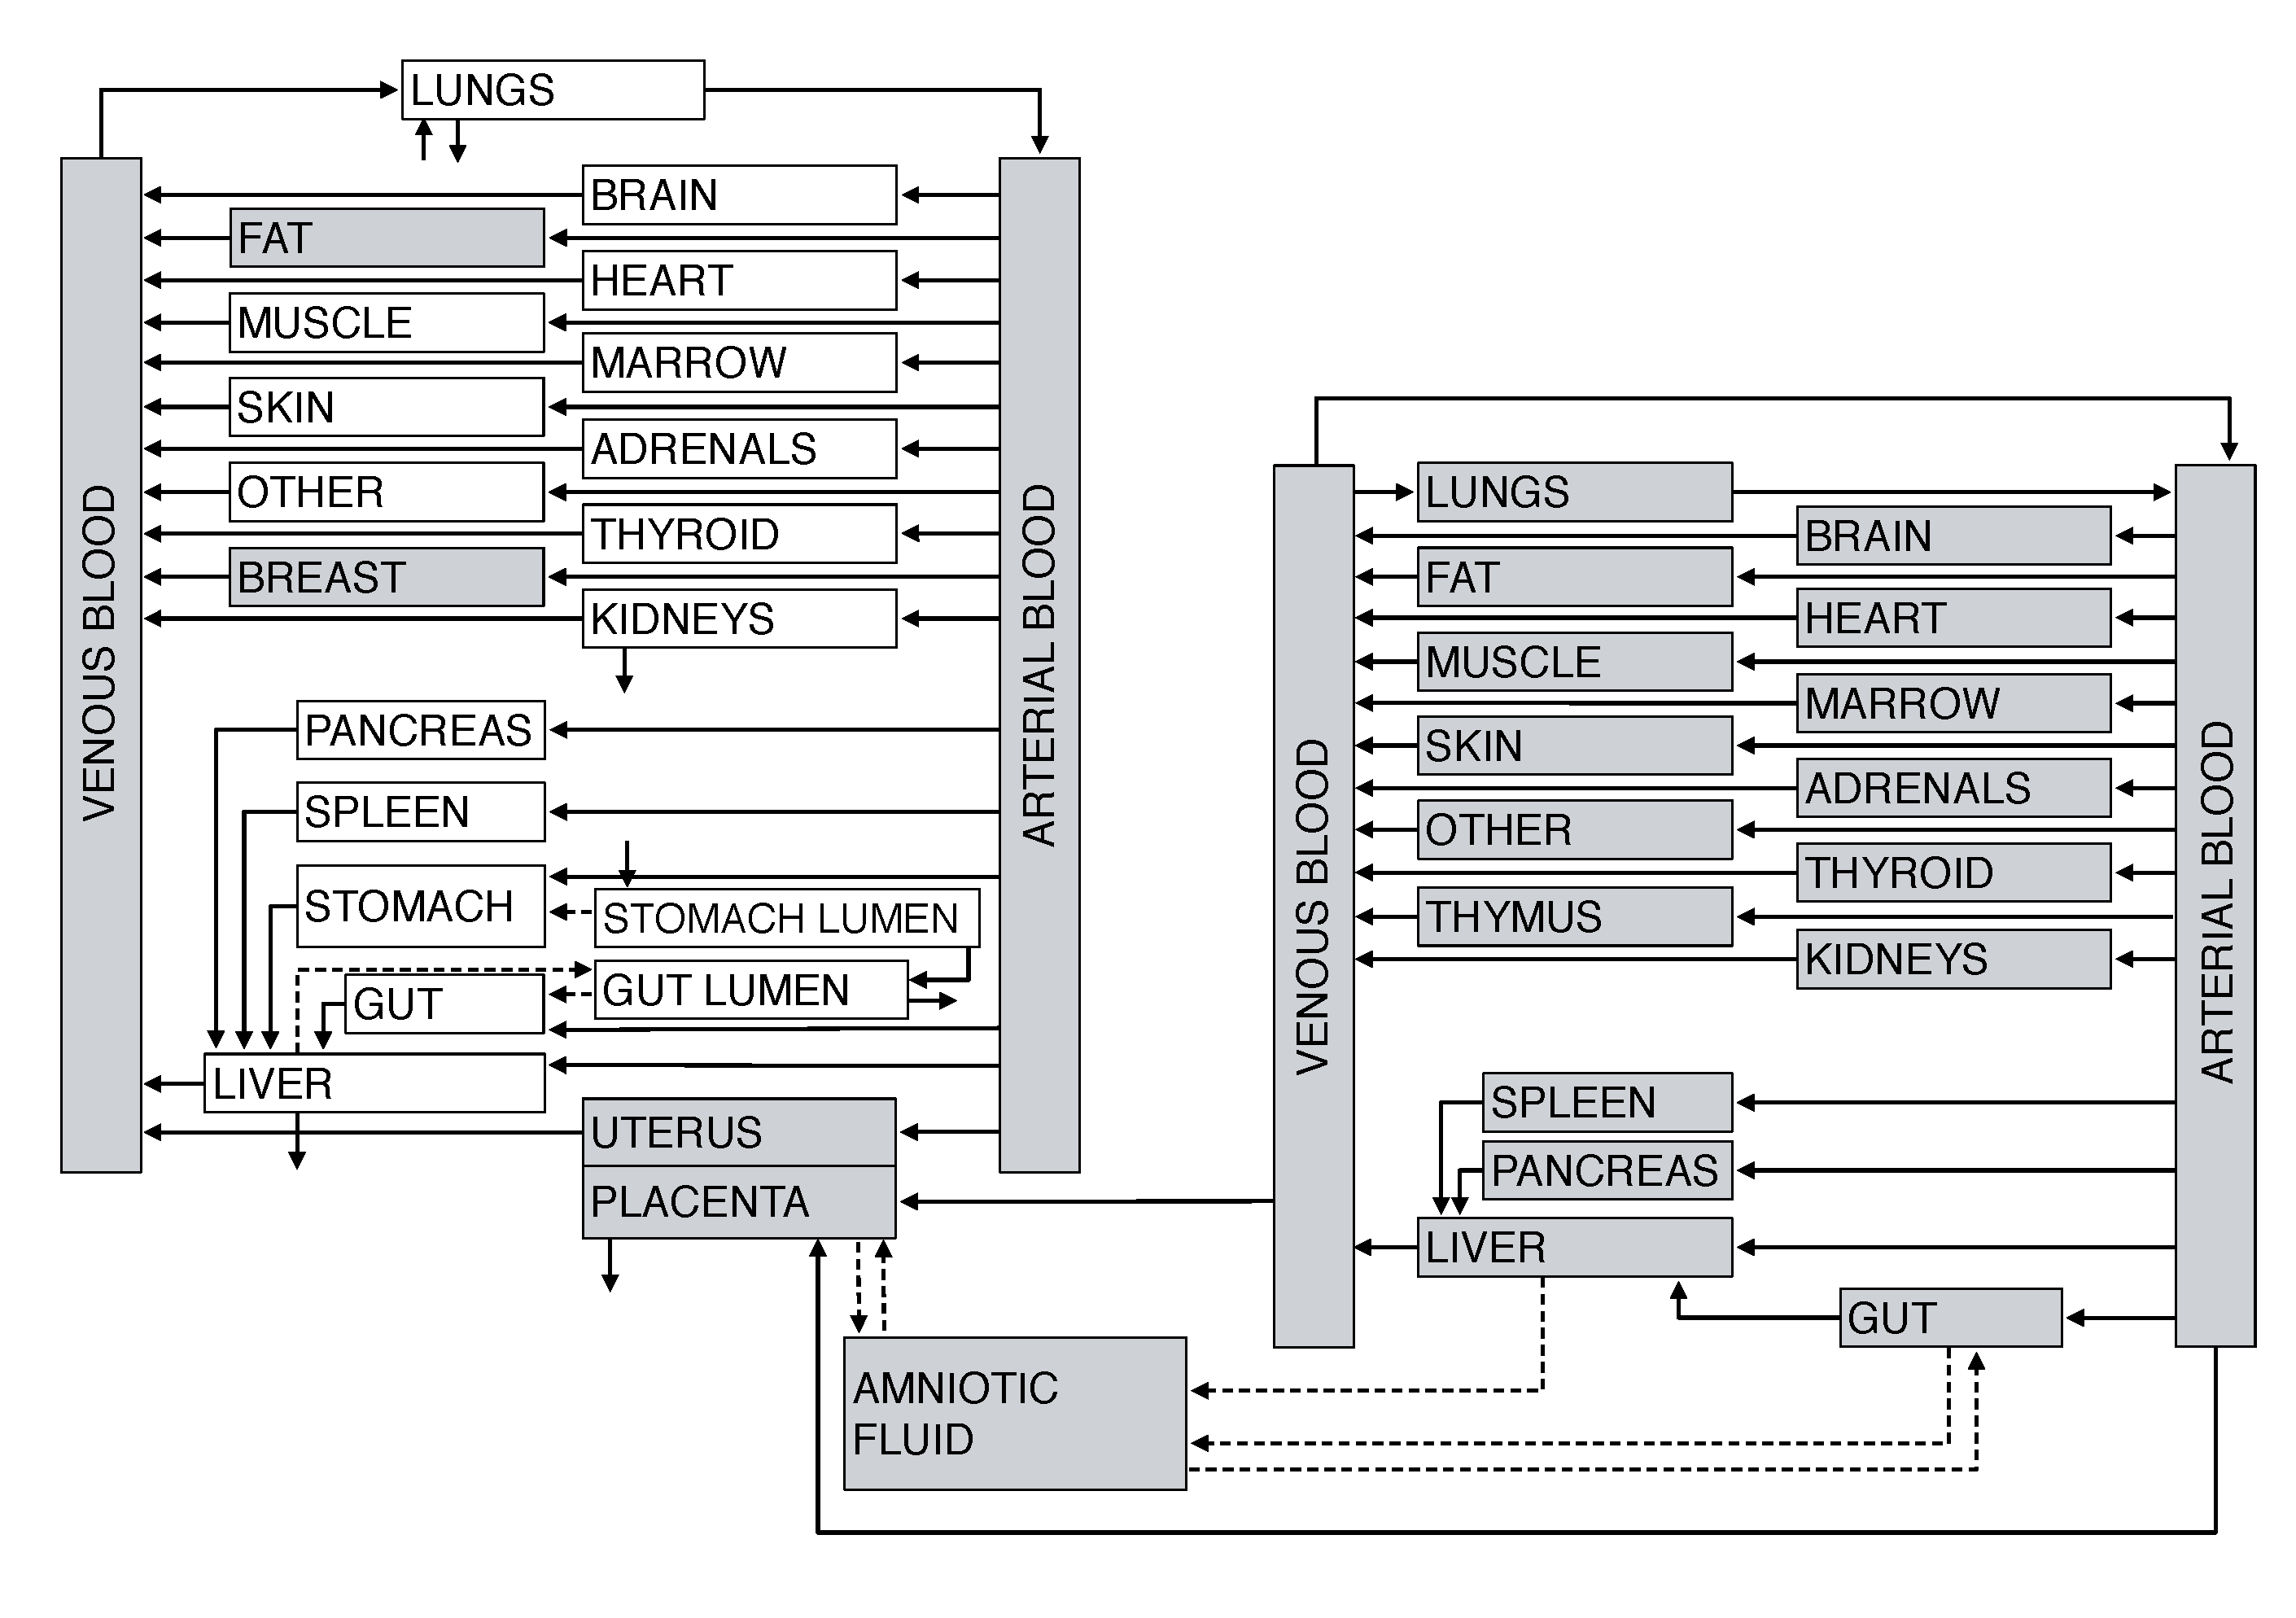
\includegraphics[width=160mm]{pics/PregnantWoman}
%  \caption{Pregnant woman PBPK model.}
%\end{figure}
%
%
%\subsection{Version 0.8.1}
%
%\subsection{Version 0.9}
%


%%%%%%%%%%%%%%%%%%%%%%%%%%%%%%%%%%%%%%%%%%%%%%%%%%%%%%%%%%%%%%%%%%%%%%%
%\section{Derivatives}
%
%Assessing Insulin Secretion by Modeling in
%Multiple-Meal Tests
%Role of Potentiation
%The second insulin secretion component [Sd(t)] represents a dynamic
%dependence of insulin secretion on the rate of change of glucose concentration.
%Sd(t) is proportional to the derivative of glucose concentration when the
%derivative is positive, and is 0 otherwise


%%%%%%%%%%%%%%%%%%%%%%%%%%%%%%%%%%%%%%%%%%%%%%%%%%%%%%%%%%%%%%%%%%%%%%
\section{Constraints}
\label{sec:constraints}

This example comes from \cite{Dalla-Man:2002bs} and illustrates how 
constraints can be declared.

\begin{align}
\int_{0}^{420} Ra \; dx = \dfrac{D f}{BW} \nonumber 
\end{align}

\lstset{language=XML}
\begin{lstlisting}
                <ct:AssignStatement op="eq">
                    <math:Integral>
                        <math:LowLimit>
                            <ct:Assign>
                                <ct:Real>0</ct:Real>
                            </ct:Assign>
                        </math:LowLimit>
                        <math:UpLimit>
                            <ct:Assign>
                                <ct:Real>420</ct:Real>
                            </ct:Assign>
                        </math:UpLimit>
                        <math:IntegrationVariable>
                            <ct:Assign>
                                <ct:SymbRef symbIdRef="t"/>
                            </ct:Assign>
                        </math:IntegrationVariable>
                        <math:IntegralArgument>
                            <ct:Assign>
                                <ct:SymbRef symbIdRef="Ra"/>
                            </ct:Assign>
                        </math:IntegralArgument>
                    </math:Integral>
                    <math:Binop op="divide">
                        <math:Binop op="times">
                            <ct:SymbRef symbIdRef="D"/>
                            <ct:SymbRef symbIdRef="f"/>
                        </math:Binop>
                        <ct:SymbRef blkIdRef="cm1" symbIdRef="BW"/>
                    </math:Binop>
                </ct:AssignStatement>
\end{lstlisting}


